\documentclass[aspectratio=169]{beamer}
\usetheme{Madrid}
\usecolortheme{default}
\usepackage{booktabs}
\usepackage{graphicx}
\usepackage{array}
\usepackage{hyperref}

\title[Toy Ontology v2]{Branch Specialization in Ordinary Attention Heads}
\subtitle{Toy Ontology v2: Structural Role Affinity, Specialization, and Modularity}
\author{Codex autonomous research checkpoint}
\date{2026-05-23}

\newcommand{\smallpath}[1]{{\tiny\texttt{\detokenize{#1}}}}
\newcommand{\dims}[1]{{\texttt{\detokenize{#1}}}}

\begin{document}

\begin{frame}
  \titlepage
\end{frame}

\begin{frame}{Checkpoint Purpose}
  \begin{itemize}
    \item User direction: keep the unit as an ordinary attention head.
    \item Question: do different-shaped attention heads make some functional roles more likely to be learned by particular head types?
    \item This round expands from a small 6-row ontology to a 20-role ontology.
    \item Every result is shown as baseline, heterogeneous result, interpretation.
  \end{itemize}
\end{frame}

\begin{frame}{Current Claim}
  \textbf{Strong current claim}
  \begin{quote}
    Heterogeneous ordinary attention-head dimensions induce structural role affinity and increase role-level specialization in this toy setting.
  \end{quote}

  \vspace{0.4cm}
  \textbf{Cautious current claim}
  \begin{quote}
    Functional modularity can improve in some layouts, but heterogeneity alone does not guarantee family-level modularity.
  \end{quote}
\end{frame}

\begin{frame}{Three Questions}
  \small
  \begin{tabular}{p{0.26\linewidth}p{0.36\linewidth}p{0.28\linewidth}}
    \toprule
    Question & What it asks & Metric here \\
    \midrule
    Structural role affinity & Which structural head type gets a role? & Top dimension, largest-dim top rate, top-dim mass \\
    Functional specialization & Is one role concentrated into one or a few heads? & Top role mass, effective heads \\
    Functional modularity & Do related roles use similar head distributions? & Family gap and ARI \\
    \bottomrule
  \end{tabular}

  \vspace{0.4cm}
  Specialization is role-level concentration. Modularity is family-level clustering. They can disagree.
\end{frame}

\begin{frame}{Ontology Hierarchy}
  \centering
  \large
  \texttt{ontology}\\
  \vspace{0.15cm}
  $\downarrow$\\
  \texttt{family}\\
  \vspace{0.15cm}
  $\downarrow$\\
  \texttt{role / subrole}\\
  \vspace{0.15cm}
  $\downarrow$\\
  \texttt{synthetic scene}\\
  \vspace{0.15cm}
  $\downarrow$\\
  \texttt{target positions}\\
  \vspace{0.15cm}
  $\downarrow$\\
  \texttt{role x head causal row}
\end{frame}

\begin{frame}{Toy Ontology v2}
  \small
  \begin{tabular}{p{0.25\linewidth}p{0.66\linewidth}}
    \toprule
    Family & Roles \\
    \midrule
    \texttt{copy\_transport} & local copy, previous token, KV lookup, duplicate token \\
    \texttt{induction} & short induction, long induction, n-gram induction, false-induction control \\
    \texttt{position\_boundary} & BOS sink, SEP sink, fixed offset, punctuation boundary \\
    \texttt{suppression\_conflict} & distractor suppression, anti-copy, wrong-key suppression, recency conflict \\
    \texttt{entity\_coreference} & repeated-name detection, pronoun antecedent, IOI name mover, negative-name control \\
    \bottomrule
  \end{tabular}

  \vspace{0.4cm}
  Total: 5 families x 4 roles = 20 measured role rows.
\end{frame}

\begin{frame}{Example Scenes}
  \scriptsize
  \begin{tabular}{p{0.22\linewidth}p{0.28\linewidth}p{0.40\linewidth}}
    \toprule
    Role & Scene & Target \\
    \midrule
    local copy & \texttt{[x, LOCAL\_SEP, x]} & At separator, predict the earlier token. \\
    KV lookup & \texttt{[KV\_SEP, k1,v1,\ldots,kq,vq]} & At query key, predict paired value. \\
    induction & \texttt{[IND, x1..x6, x1..x6]} & On second copy, predict continuation from first copy. \\
    recency conflict & \texttt{[key, old, key, recent, key, old]} & Prefer older value over closer recent value. \\
    IOI name mover & \texttt{[A,B,A,IOI\_QUERY,B]} & Predict non-repeated name. \\
    \bottomrule
  \end{tabular}

  \vspace{0.35cm}
  Full 20-role examples are in \smallpath{data/role_dataset_examples.json}.
\end{frame}

\begin{frame}{Literature Anchors}
  \scriptsize
  \begin{tabular}{p{0.32\linewidth}p{0.22\linewidth}p{0.36\linewidth}}
    \toprule
    Source & Venue / year & Roles motivated \\
    \midrule
    Clark et al., BERT attention & BlackboxNLP at ACL 2019 & delimiter, fixed position, syntax, coreference \\
    Voita et al., specialized heads & ACL 2019 & specialized, positional, syntactic, rare-token heads \\
    Elhage et al., Transformer Circuits & Transformer Circuits 2021 & QK/OV, previous-token heads, circuits \\
    Olsson et al., induction heads & Transformer Circuits / arXiv 2022 & induction and previous-token composition \\
    Wang et al., IOI circuit & ICLR 2023 & name movers, negative heads, duplicate-token roles \\
    McDougall et al., copy suppression & arXiv/OpenReview 2023; BlackboxNLP 2024 & copy suppression and negative copy effects \\
    \bottomrule
  \end{tabular}
\end{frame}

\begin{frame}{Experiment Settings}
  \small
  \begin{tabular}{ll}
    \toprule
    Item & Value \\
    \midrule
    Unit & ordinary attention head \\
    Model & tiny decoder-only transformer \\
    Dataset & one synthetic 20-role next-token sequence generator \\
    Total attention dimension & 128 in every config \\
    Seeds & 1, 2, 3, 4, 5 \\
    Steps & 1600 \\
    Eval examples & 512 \\
    Measurement & single-head ablation, role x head causal matrix \\
    \bottomrule
  \end{tabular}
\end{frame}

\begin{frame}{Configs}
  \scriptsize
  \begin{tabular}{p{0.30\linewidth}p{0.24\linewidth}p{0.36\linewidth}}
    \toprule
    Config & Head dims & Purpose \\
    \midrule
    \texttt{uniform4} & \dims{[32,32,32,32]} & four-head uniform baseline \\
    \texttt{uniform2} & \dims{[64,64]} & strong fewer/wider uniform baseline \\
    \texttt{hetero4\_unique\_mild} & \dims{[16,24,40,48]} & mild four-head heterogeneity \\
    \texttt{hetero4\_unique\_64} & \dims{[8,16,40,64]} & one 64-dim structural type \\
    \texttt{hetero4\_unique\_extreme} & \dims{[8,16,24,80]} & extreme four-head imbalance \\
    \texttt{hetero2\_unique\_mild} & \dims{[48,80]} & mild two-head heterogeneity \\
    \texttt{hetero2\_unique\_mid} & \dims{[32,96]} & medium two-head heterogeneity \\
    \texttt{hetero2\_unique\_extreme} & \dims{[16,112]} & extreme two-head heterogeneity \\
    \bottomrule
  \end{tabular}
\end{frame}

\begin{frame}{Learnability Check}
  \small
  \begin{tabular}{lcc}
    \toprule
    Config & Mean role accuracy & Min role accuracy \\
    \midrule
    \texttt{uniform4} & 1.000 & 0.998 \\
    \texttt{uniform2} & 0.999 & 0.991 \\
    \texttt{hetero4\_unique\_mild} & 1.000 & 0.999 \\
    \texttt{hetero4\_unique\_64} & 1.000 & 0.999 \\
    \texttt{hetero4\_unique\_extreme} & 1.000 & 0.999 \\
    \texttt{hetero2\_unique\_mild} & 1.000 & 0.999 \\
    \texttt{hetero2\_unique\_mid} & 1.000 & 0.996 \\
    \texttt{hetero2\_unique\_extreme} & 1.000 & 0.997 \\
    \bottomrule
  \end{tabular}

  \vspace{0.3cm}
  Interpretation: comparisons are not driven by failed training.
\end{frame}

\begin{frame}{Q1: Structural Role Affinity}
  \scriptsize
  \begin{tabular}{lccc}
    \toprule
    Hetero config & Chance largest top & Observed largest top & Mean top-dim mass \\
    \midrule
    \dims{[16,24,40,48]} & 0.25 & 0.50 & 0.759 \\
    \dims{[8,16,40,64]} & 0.25 & 0.65 & 0.821 \\
    \dims{[8,16,24,80]} & 0.25 & 0.82 & 0.912 \\
    \dims{[48,80]} & 0.50 & 0.66 & 0.839 \\
    \dims{[32,96]} & 0.50 & 0.82 & 0.871 \\
    \dims{[16,112]} & 0.50 & 0.94 & 0.937 \\
    \bottomrule
  \end{tabular}

  \vspace{0.35cm}
  Interpretation: larger structural head types attract roles far above chance, and the effect strengthens with imbalance.
\end{frame}

\begin{frame}{Q2: Functional Specialization}
  \scriptsize
  \begin{tabular}{lcc}
    \toprule
    Config & Specialization & Effective heads \\
    \midrule
    \texttt{uniform4} & 0.733 & 2.400 \\
    \texttt{uniform2} & 0.684 & 2.166 \\
    \texttt{hetero4\_unique\_mild} & 0.726 & 2.206 \\
    \texttt{hetero4\_unique\_64} & 0.776 & 1.906 \\
    \texttt{hetero4\_unique\_extreme} & 0.849 & 1.522 \\
    \texttt{hetero2\_unique\_mild} & 0.782 & 1.802 \\
    \texttt{hetero2\_unique\_mid} & 0.776 & 1.692 \\
    \texttt{hetero2\_unique\_extreme} & 0.780 & 1.636 \\
    \bottomrule
  \end{tabular}

  \vspace{0.35cm}
  Interpretation: heterogeneity generally concentrates each role into fewer causal heads.
\end{frame}

\begin{frame}{Q3: Functional Modularity}
  \scriptsize
  \begin{tabular}{lcc}
    \toprule
    Config & Family gap & ARI \\
    \midrule
    \texttt{uniform4} & 0.153 & 0.149 \\
    \texttt{uniform2} & 0.117 & 0.108 \\
    \texttt{hetero4\_unique\_mild} & 0.137 & 0.082 \\
    \texttt{hetero4\_unique\_64} & 0.127 & 0.113 \\
    \texttt{hetero4\_unique\_extreme} & 0.138 & 0.111 \\
    \texttt{hetero2\_unique\_mild} & 0.128 & 0.112 \\
    \texttt{hetero2\_unique\_mid} & 0.151 & 0.159 \\
    \texttt{hetero2\_unique\_extreme} & 0.050 & 0.039 \\
    \bottomrule
  \end{tabular}

  \vspace{0.35cm}
  Interpretation: modularity is not automatic. The best two-head hetero layout is promising, but extreme imbalance can collapse family structure.
\end{frame}

\begin{frame}{Aggregate Metric Plot}
  \centering
  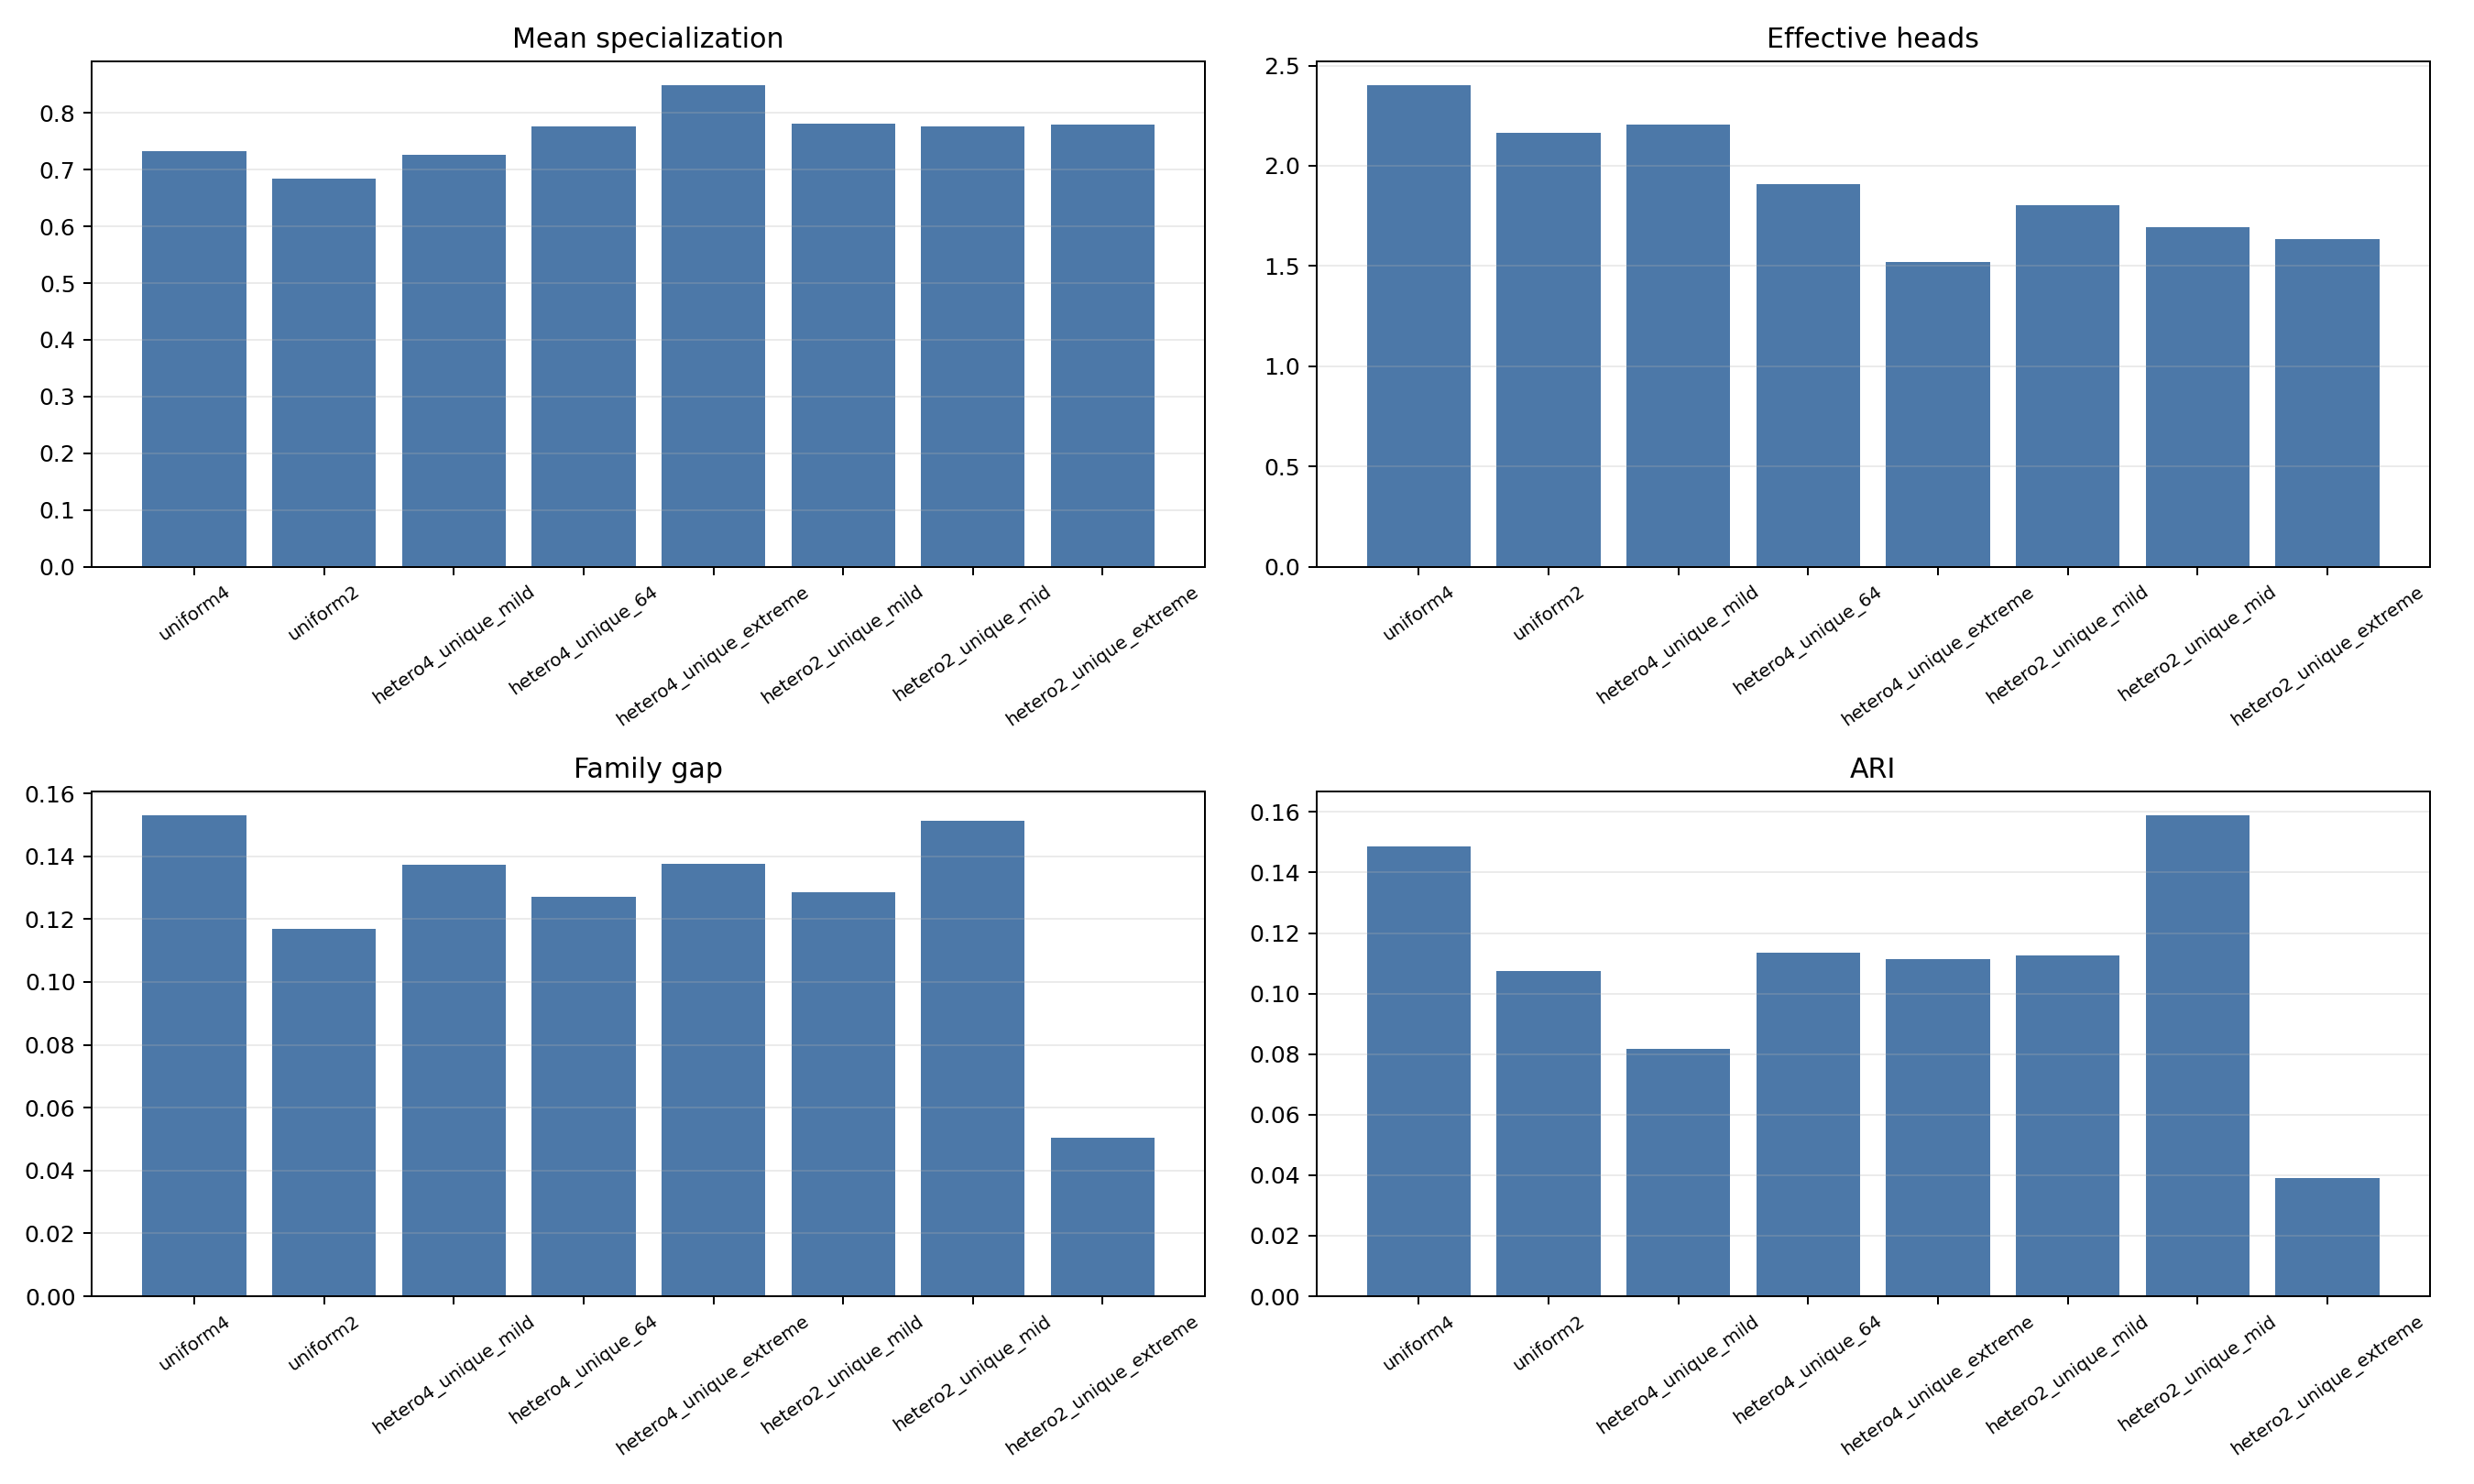
\includegraphics[width=0.90\linewidth]{../figures/full_config_metric_bars.png}
\end{frame}

\begin{frame}{Family Specialization Heatmap}
  \centering
  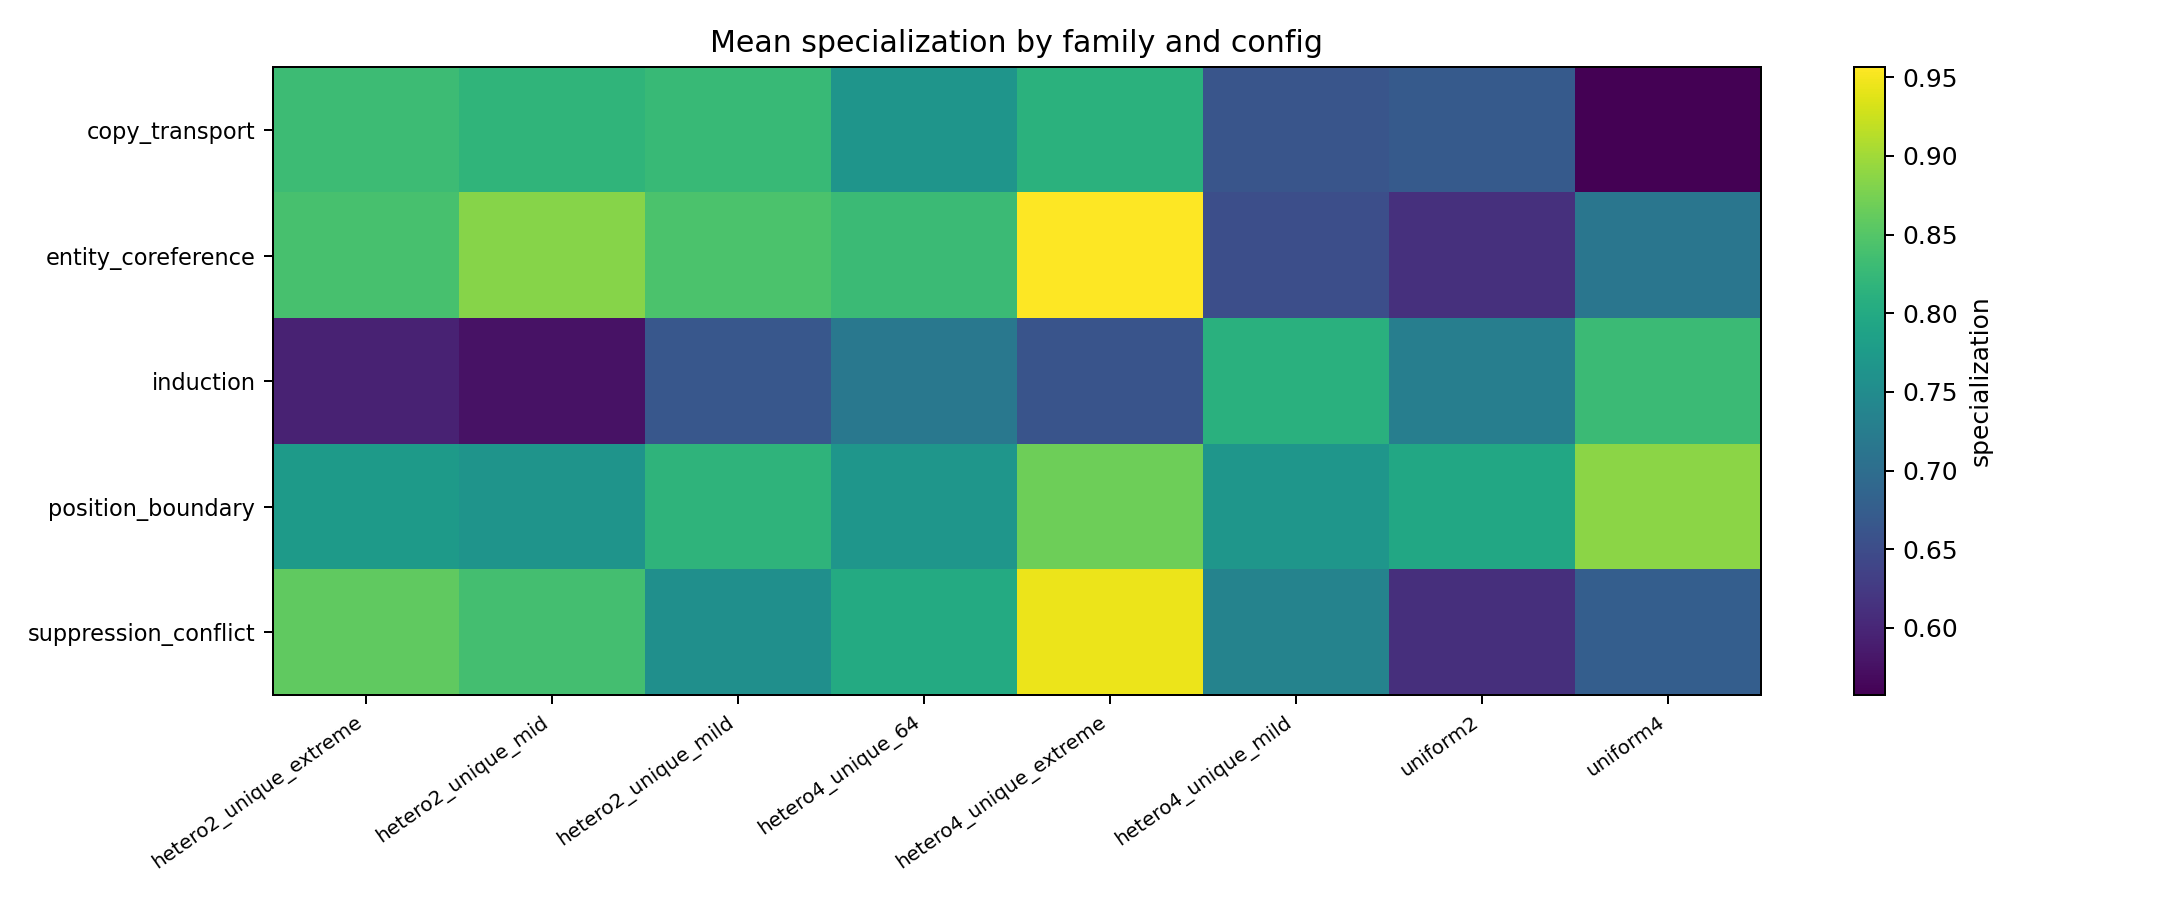
\includegraphics[width=0.90\linewidth]{../figures/full_family_specialization_heatmap.png}
\end{frame}

\begin{frame}{Layout Control}
  \small
  The key check: if a role only likes head index H3, moving the 64-dim head should not move the role.

  \vspace{0.3cm}
  Layouts tested:
  \begin{itemize}
    \item \dims{[8,16,40,64]}
    \item \dims{[64,8,16,40]}
    \item \dims{[8,64,16,40]}
    \item \dims{[8,16,64,40]}
  \end{itemize}
\end{frame}

\begin{frame}{Layout Results}
  \scriptsize
  \begin{tabular}{lcccc}
    \toprule
    Layout & 64 position & Largest-top rate & Family gap & ARI \\
    \midrule
    \dims{[8,16,40,64]} & H3 & 0.65 & 0.127 & 0.113 \\
    \dims{[64,8,16,40]} & H0 & 0.68 & 0.100 & 0.089 \\
    \dims{[8,64,16,40]} & H1 & 0.67 & 0.086 & 0.096 \\
    \dims{[8,16,64,40]} & H2 & 0.60 & 0.186 & 0.189 \\
    \bottomrule
  \end{tabular}

  \vspace{0.35cm}
  Interpretation: the 64-dim preference persists when the 64-dim head moves, but family modularity is layout-sensitive.
\end{frame}

\begin{frame}{Which Roles Followed The 64-Dim Type?}
  \scriptsize
  \begin{tabular}{lcc}
    \toprule
    Role & 64-dim top cases & Rate \\
    \midrule
    \texttt{local\_copy} & 20/20 & 1.00 \\
    \texttt{negative\_name\_control} & 19/20 & 0.95 \\
    \texttt{recency\_conflict} & 19/20 & 0.95 \\
    \texttt{wrong\_key\_suppression} & 19/20 & 0.95 \\
    \texttt{pronoun\_antecedent} & 18/20 & 0.90 \\
    \texttt{kv\_lookup} & 17/20 & 0.85 \\
    \texttt{simple\_ioi\_name\_mover} & 17/20 & 0.85 \\
    \bottomrule
  \end{tabular}

  \vspace{0.35cm}
  Some induction and boundary roles were less 64-locked. This is evidence for role-specific affinity, not just universal collapse.
\end{frame}

\begin{frame}{Interpretation}
  \small
  \begin{tabular}{p{0.32\linewidth}p{0.18\linewidth}p{0.40\linewidth}}
    \toprule
    Claim & Status & Reason \\
    \midrule
    Heterogeneous dimensions create structural role affinity & Strong toy evidence & Above-chance largest-head selection and layout controls \\
    Heterogeneous dimensions increase specialization & Strong toy evidence & Higher top-role mass and fewer effective heads \\
    Heterogeneous dimensions create modularity & Mixed & Some layouts improve, others do not; extreme imbalance hurts \\
    Toy ontology maps to real LM roles & Not proven yet & Literature-grounded roles, but synthetic dataset \\
    \bottomrule
  \end{tabular}
\end{frame}

\begin{frame}{Decision}
  \large
  Continue the project.

  \vspace{0.5cm}
  \normalsize
  The evidence is strong enough for the structural-affinity and specialization story.

  \vspace{0.25cm}
  The modularity story should be treated as a separate research question, not as something automatically implied by heterogeneous dimensions.
\end{frame}

\begin{frame}{Next Steps}
  \small
  \begin{enumerate}
    \item Extend layout controls for the best modularity layout \dims{[8,16,64,40]}.
    \item Add more induction and position-boundary subroles because they behave differently from copy/conflict roles.
    \item Run real-model validation with ordinary pretrained heads: local copy, induction, delimiter/BOS, copy suppression, and IOI-style probes.
    \item Add bootstrap confidence intervals or permutation tests before paper drafting.
    \item Keep future reporting format: baseline result, heterogeneous result, interpretation.
  \end{enumerate}
\end{frame}

\begin{frame}[fragile]{Provenance}
  \scriptsize
  Main memo:
  \begin{verbatim}
doc/experiments/phase3/phase3_toy_role_ontology_v2.md
  \end{verbatim}
  Main result root:
  \begin{verbatim}
results/phase3_toy_role_ontology_v2_full_1600_20260523
  \end{verbatim}
  Layout control root:
  \begin{verbatim}
results/phase3_toy_role_ontology_v2_layout_1600_20260523
  \end{verbatim}
  Scripts:
  \begin{verbatim}
scripts/toy_role_ontology_v2_head_dim_intervention.py
scripts/analyze_role_ontology_v2.py
  \end{verbatim}
\end{frame}

\begin{frame}[fragile]{Reproduction Commands}
  \tiny
  \begin{verbatim}
python scripts/toy_role_ontology_v2_head_dim_intervention.py \
  --role-set v2_full \
  --configs uniform4 uniform2 hetero4_unique_mild hetero4_unique_64 \
    hetero4_unique_extreme hetero2_unique_mild hetero2_unique_mid \
    hetero2_unique_extreme \
  --seeds 1 2 3 4 5 --steps 1600 --batch-size 128 \
  --eval-examples 512 \
  --output-dir results/phase3_toy_role_ontology_v2_full_1600_20260523

python scripts/analyze_role_ontology_v2.py \
  results/phase3_toy_role_ontology_v2_full_1600_20260523 \
  --title "Toy Ontology v2 Full 20-Role Sweep"
  \end{verbatim}
\end{frame}

\end{document}
